\chapter{时域分析法}
\thispagestyle{empty}
\section{时域分析基础}
 \subsection{时域分析法的特点}
 \begin{itemize}
 	\item 时域分析法是根据系统的微分方程,以Laplace变换作为数学工具解出控制系统的时间响应
 	\item 依据响应的表达式及时间响应曲线来分析系统的控制性能:稳定性、快速性、平稳性、准确性等
 	\item 找出系统的结构、参数与这些性能之间的关系
 	\item 时域分析法是一种直接分析法,也是一种比较准确的方法,可以提供系统时间响应的全部信息
 \end{itemize}
 
 \subsection{典型初始状态}
在$t = 0$时,系统处于静止状态,即
\begin{align}
	c(0^-) = \left.\dfrac{\d c(t)}{\d t}\right|_{t = 0} = \left. \dfrac{\d^2 c(t)}{\d t^2}\right|_{t=0} = \cdots = 0
\end{align}

\subsection{典型外作用}
\noindent 1. \dy[单位跃阶作用$1(t)$]{DWYJZY}
\begin{align}
	1(t) = 
	\begin{cases}
		0, & t<0 \\
		1, & t \ge 0
	\end{cases}\\[0.5em]
\mathcal{L}\big[1(t)\big] = \dfrac{1}{s}
\end{align}

\noindent 2. \dy[单位斜坡作用$t \cdot 1(t)$]{DWXPZY}
\begin{align}
	t \cdot 1(t) = 
	\begin{cases}
		0, & t<0 \\
		t, & t \ge 0
	\end{cases}\\[0.5em]
	\mathcal{L}\big[t \cdot 1(t)\big] = \dfrac{1}{s^2}
\end{align}

\noindent 3. \dy[单位脉冲作用$\delta (t)$]{DWMCZY}
\begin{align}
	\delta (t) = 
	\begin{cases}
		\infty, & t=0 \\
		0, & t \neq 0
	\end{cases}\\[0.5em]
	\mathcal{L}\big[\delta (t)\big] = 1
\end{align}

\noindent 4. \dy[正弦作用$A\sin(\omega t) \cdot 1(t)$]{ZXZY}
\begin{align}
	A\sin(\omega t) \cdot 1(t) = 
	\begin{cases}
		0, & t<0 \\
		A\sin(\omega t), & t \ge 0
	\end{cases}\\[0.5em]
	\mathcal{L}\big[A\sin(\omega t) \cdot 1(t)\big] = \dfrac{A \omega }{s^2 + \omega^2}
\end{align}

\subsection{典型时间响应}
\noindent 1. \dy[单位跃阶响应$h(t)$]{DWYJXY}
\par 系统在单位跃阶输入作用下的响应,常用$h(t)$表示,若系统的闭环传递函数为$\varPhi (s)$,则
\begin{align}
	H(s) = \varPhi(s) \cdot R(s) = \varPhi(s) \cdot \dfrac{1}{s} \notag \\[0.5em]
	h(t) = \mathcal{L}^{-1}\big[H(s)\big]\label{XY1}
\end{align}

\noindent 2. \dy[单位斜坡响应$c_{\text{t}}(t)$]{DWXPXY}
\par 系统在单位斜坡输入作用下的响应,常用$c_{\text{t}}(t)$表示,若系统的闭环传递函数为$\varPhi (s)$,则
\begin{align}
	C_{\text{t}}(s) = \varPhi(s) \cdot R(s) = \varPhi(s) \cdot \dfrac{1}{s^2} \notag \\[0.5em]
	c_{\text{t}}(t) = \mathcal{L}^{-1}\big[C_\text{t}(s)\big]\label{XY2}
\end{align}

\noindent 3. \dy[单位脉冲响应$k(t)$]{DWMCXY}
\par 系统在单位脉冲输入作用下的响应,常用$k(t)$表示,若系统的闭环传递函数为$\varPhi (s)$,则
\begin{align}
	K(s) = \varPhi(s) \cdot R(s) = \varPhi(s) \notag \\[0.5em]
	k(t) = \mathcal{L}^{-1}\big[K(s)\big]\label{XY3}
\end{align}

\noindent 4. \dyn{三种响应之间的关系}
\par 由式\eqref{XY1},\eqref{XY2},\eqref{XY3}可得
\begin{align}
	H(s) = \varPhi(s) \dfrac{1}{s} =K(s) \dfrac{1}{s} \\[0.5em]
	C_\text{t}(s) = \varPhi(s) \dfrac{1}{s^2} = H(s)\dfrac{1}{s}
\end{align}
即
\begin{align}
	K(s)=sH(s)\\[0.5em]
	H(s) = sC_\text{t} (s)
\end{align}
从而得到时域表达式为
\begin{align}
	k(t) = \dfrac{\d h(t)}{\d t}\\[0.5em]
	h(t) = \dfrac{\d c_{\text{t}}(t)}{\d t}
\end{align}

\subsection{阶跃响应的性能指标}
\begin{figure}[!htp]
	\centering
	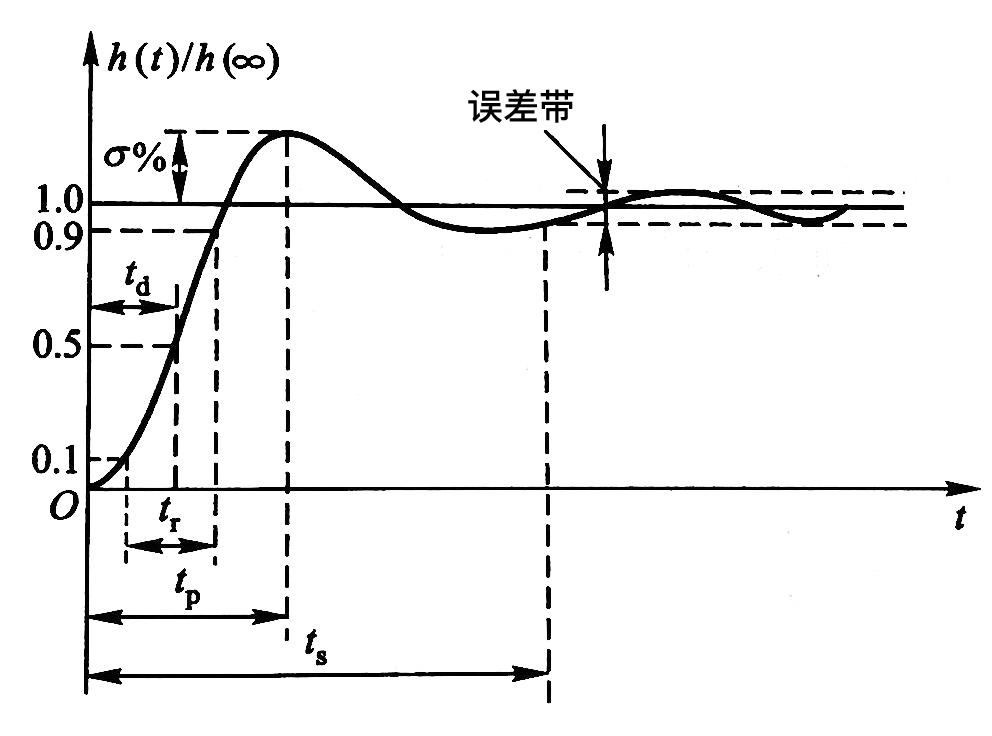
\includegraphics[width=0.5\linewidth]{pic/性能指标.jpg}
	\caption{控制系统的典型单位阶跃响应}
	\label{控制系统的典型单位阶跃响应}
\end{figure}
\noindent 控制系统的常用指标,如图\ref{控制系统的典型单位阶跃响应}.
\begin{itemize}
	\item 系统的快速性指标
	\begin{itemize}
		\item 反映系统响应初始阶段的快慢
		\begin{itemize}
			\item \dy[延迟时间$t_{\text{d}}$]{YCSJ}\quad 单位阶跃曲线$h(t)$上升到其稳态值的$50 \%$所需要的时间。
			\item \dy[上升时间$t_{\text{r}}$]{SSSJ}\quad 单位阶跃曲线$h(t)$从稳态值的$10\%$上升到$90\%$所需要的时间。
			\item \dy[峰值时间$t_{\text{p}}$]{FZSJ}\quad 单位阶跃曲线$h(t)$超过其稳态值而达到第一个峰值所需要的时间。
		\end{itemize}
		\item 反映系统过渡过程持续的时间
		\begin{itemize}
			\item \dy[调节时间$t_{\text{s}}$]{TJSJ}\quad 单位阶跃曲线$h(t)$的稳态值附近,取$\pm 5 \%$(或$\pm 2\%$)作为误差带,响应曲线达到并不再超出该误差带的最小时间,标志着过渡过程结束,系统的响应进入稳态过程。
		\end{itemize}
	\end{itemize}
	\item 系统的平稳性指标
	\begin{itemize}
		\item \dy[超调量$\sigma \, \%$]{CTL}\quad 在响应过程中,超出稳态值的最大偏离量和稳态值之比,即
		\begin{align}
			\sigma \,\% = \dfrac{h(t_{\text{p}})-h(\infty)}{h(\infty)} \times 100 \%
		\end{align}
	\end{itemize}
	\item 系统的稳态精度指标
	\begin{itemize}
		\item \dy[稳态误差$e_{\text{ss}}$]{WTWC}\quad 当时间$t$趋于无穷时,系统单位阶跃响应的实际值(稳态值)与期望值(一般为输入量$1(t)$)之差,即
		\begin{align}
			e_{\text{ss}} = 1 - h(\infty)
		\end{align}
	\end{itemize}
\end{itemize}

\section{一阶系统分析与计算}
\subsection{一阶系统的数学模型}
一阶系统的微分方程为
\begin{align}
	T\dfrac{\d c(t)}{\d t} + c(t) = r(t)
	\label{一阶模型1}
\end{align}
其中,
\begin{myitemize}
	\item $c(t)$ \quad 输出量\vspace*{-0.5em}
	\item $r(t)$ \quad 输入量\vspace*{-0.5em}
	\item $T$ \quad 时间常数\vspace*{0.3em}
\end{myitemize}

\begin{figure}[!htb]
	\centering
	\begin{tikzpicture}[circuit ee IEC,node distance=1.2cm]
		\node[bulb] (A)  [draw, inner sep=5pt,label=-80:$-$] {};
		\node (B) [draw, inner sep =4pt,right of = A, node distance = 1.5cm]{$\,\dfrac{K}{s}\,$};
		
		\draw[arrows={-Stealth}] (-1cm,0cm) -- (A)node[near start, above = 0cm]{$R(s)$};
		\draw [arrows={-Stealth}] (A) -- (B);
		\draw[arrows={-Stealth}] (B) -- (3cm,0cm)node[near end, above =0cm]{$C(s)$};
		\draw[arrows={-Stealth}] (2.3cm,0cm) -- +(0cm, -1cm) -- (0cm,-1cm) -- (A);
	\end{tikzpicture}
\caption{一阶系统结构图}
\label{一阶系统}
\end{figure}

一阶系统的结构图如图\ref{一阶系统}.其闭环传递函数为
\begin{align}
	\varPhi (s) = \dfrac{C(s)}{R(s)} = \dfrac{1}{\dfrac{1}{K} + s} =\dfrac{1}{Ts +1}
	\label{一阶模型2}
\end{align}
其中,$T = \dfrac{1}{K}$.
\vspace*{0.5em}

式\eqref{一阶模型1},\eqref{一阶模型2}称为\dy[一阶系统的数学模型]{YJXTDSXMX}。\dy[时间常数$T$]{SJCS}是反映系统惯性的一个主要参数,故一阶系统也称为\dy[惯性环节]{GXHJ}。
\vspace*{0.5em}
\subsection{一阶系统的单位阶跃模型}
由单位阶跃输入的Laplace变换
\begin{align}
	R(s) = \dfrac{1}{s}\notag
\end{align}
结合式\eqref{一阶模型2}可得
\begin{align}
	C(s) = \varPhi(s) R(s) = \dfrac{1}{Ts+1}\cdot\dfrac{1}{s}\notag
\end{align}
取反变换,得
\begin{align}
	h(t) = \mathcal{L}^{-1}\left[\dfrac{1}{Ts+1}\cdot\dfrac{1}{s}\right] =  \mathcal{L}^{-1}\left[\dfrac{1}{s} - \dfrac{1}{s + \dfrac{1}{T}}\right] \notag
\end{align}
所以
\begin{align}
	h(t) &= 1 - \e ^{ -{\textstyle \frac{1}{T}} t}\\
			&= c_{\text{ss}} + c_{\text{tt}}
\end{align}
其中,$c_{\text{ss}} = 1$代表稳态分量;$c_{\text{tt}}$代表瞬态分量。

\noindent 特点:\vspace*{-0.5em}
\begin{itemize}
	\item 曲线\\
	\hspace*{2em}当$t \to \infty,c_{\text{tt}}\to 0$,所以一阶系统的单位阶跃响应曲线是一条由零开始按指数规律上升并最终趋于1的曲线。 
	\item 时间常数$T$\\
	\hspace*{2em}时间常数$T$是表征响应特征的唯一参数,它与输出值有确定的关系
	\begin{align}
		h(T) &= 0.632\notag\\
		h(2T) &= 0.865\notag\\
		h(3T) &= 0.950 \notag\\
		h(4T) &= 0.982\notag
	\end{align}
	可以用实验方法,根据这些值鉴别和确定被测系统是否为一阶系统及时间常数$T$。
	\item 超调量\\
	\hspace*{2em} 一阶系统阶跃响应没有超调量。
	\item 调节时间
	\begin{align}
		t_{\text{s}} = 3 T,\mbox{对应}5\% \mbox{误差带}\\
		t_{\text{s}} = 4 T,\mbox{对应}2\% \mbox{误差带}
	\end{align}
	所以,系统的时间常数$T$越小,调节时间$t_{\text{s}}$越小,响应曲线很快就能接近稳定值。
	\item 稳态误差\\
	\hspace*{2em}系统的单位阶跃响应是没有稳定误差的,即
	\begin{align}
		e_{\text{ss}} = 1 - h(\infty) = 0
	\end{align}
\end{itemize}

\section{二阶系统分析与计算}
\subsection{二阶系统的数学模型}
二阶微分方程
\begin{align}
	\dfrac{\d^2 c(t)}{\d t^2} + 2 \zeta \omega_\n \dfrac{\d c(t)}{\d t} + \omega_\n^2c(t) = \omega_\n^2r(t), \quad \omega_\n >0
\end{align}
其中,
\begin{myitemize}
	\item $r(t)$\quad 系统的输入量\vspace*{-0.5em}
	\item $c(t)$\quad 系统的输出量\vspace*{-0.5em}
	\item $\omega_\n\,$ \quad \dy[无阻尼的自然频率]{WZNDZRPL}或\dy[固有频率]{GYPL}\vspace*{-0.5em}
	\item $\zeta$\quad\quad \dy[阻尼比]{ZNB}\vspace*{0.3em}
\end{myitemize}

\noindent 作Laplace变换,得到二阶系统的传递函数为
\begin{align}
	\varPhi(s) = \dfrac{\omega_\n^2}{s^2 + 2 \zeta \omega_\n s + \omega_\n^2}
\end{align}
对应二阶系统的结构图如图\ref{二阶系统}.

\dy[二阶系统的特征方程]{EJXTDTZFC}为
\begin{align}
	s^2 + 2 \zeta \omega_\n s + \omega_\n^2 = 0
\end{align}

\begin{figure}[!htb]
	\centering
	\begin{tikzpicture}[circuit ee IEC,node distance=1.2cm]
		\node[bulb] (A)  [draw, inner sep=5pt,label=-80:$-$] {};
		\node (B) [draw, inner sep =4pt,right of = A, node distance = 2cm]{$\,\dfrac{\omega_\n^2}{s^2 + 2 \zeta \omega_\n s}\,$};
		
		\draw[arrows={-Stealth}] (-1cm,0cm) -- (A)node[near start, above = 0cm]{$R(s)$};
		\draw [arrows={-Stealth}] (A) -- (B);
		\draw[arrows={-Stealth}] (B) -- (4cm,0cm)node[near end, above =0cm]{$C(s)$};
		\draw[arrows={-Stealth}] (3.5cm,0cm) -- +(0cm, -1cm) -- (0cm,-1cm) -- (A);
	\end{tikzpicture}
	\caption{二阶系统结构图}
	\label{二阶系统}
\end{figure}

方程的特征根为
\begin{align}
	s_{1,2} = - \zeta \omega_\n \pm \omega_\n \sqrt{\zeta^2 -1}
	\label{二阶3}
\end{align}
由式\eqref{二阶3}分析可得:
\begin{itemize}
	\item $0 < \zeta < 1$ \quad 特征方程有一对实部为负的共轭复根$s_{1,2} = - \zeta \omega_\n \pm \j \omega_\n\sqrt{1 - \zeta^2}$,称为\dy[欠阻尼状态]{QZNZT}。\vspace*{-0.5em}
	\item $\zeta = 1$\quad 特征方程有两个相等的负实根,称为\dy[临界阻尼状态]{LJZNZT}。\vspace*{-0.5em}
	\item $\zeta > 1$\quad 特征方程有两个不相等的负实根,称为\dy[过阻尼状态]{GZNZT}。\vspace*{-0.5em}
	\item $\zeta = 0$ \quad 特征方程有一对纯虚根,称为\dy[零阻尼状态]{LZNZT}。\vspace*{-0.5em}
	\item $\zeta < 0$\quad 特征方程有两个正实部的根,称为\dy[负阻尼状态]{FZNZT}。
\end{itemize}

\warn[
各个$\zeta$系统的特点
\begin{itemize}
	\item 欠阻尼状态$(0< \zeta <1)$系统的时间响应具有振荡性质
	\item 临界阻尼$(\zeta = 1)$和过阻尼状态$(\zeta > 1)$,系统的时间响应均无振荡
	\item 零阻尼状态$(\zeta = 0)$系统的时间响应为持续的等幅振荡
	\item 负阻尼状态$(\zeta < 0)$的系统是不稳定的
	\item $\zeta$的取值不同,二阶系统{\dy[闭环极点]{BHJD}}(即特征方程的根)在$s$平面上的分布也不同,如图\ref{二阶系统平面}.
\end{itemize}
{
	\vspace*{-0.5em}
	\begin{center}
		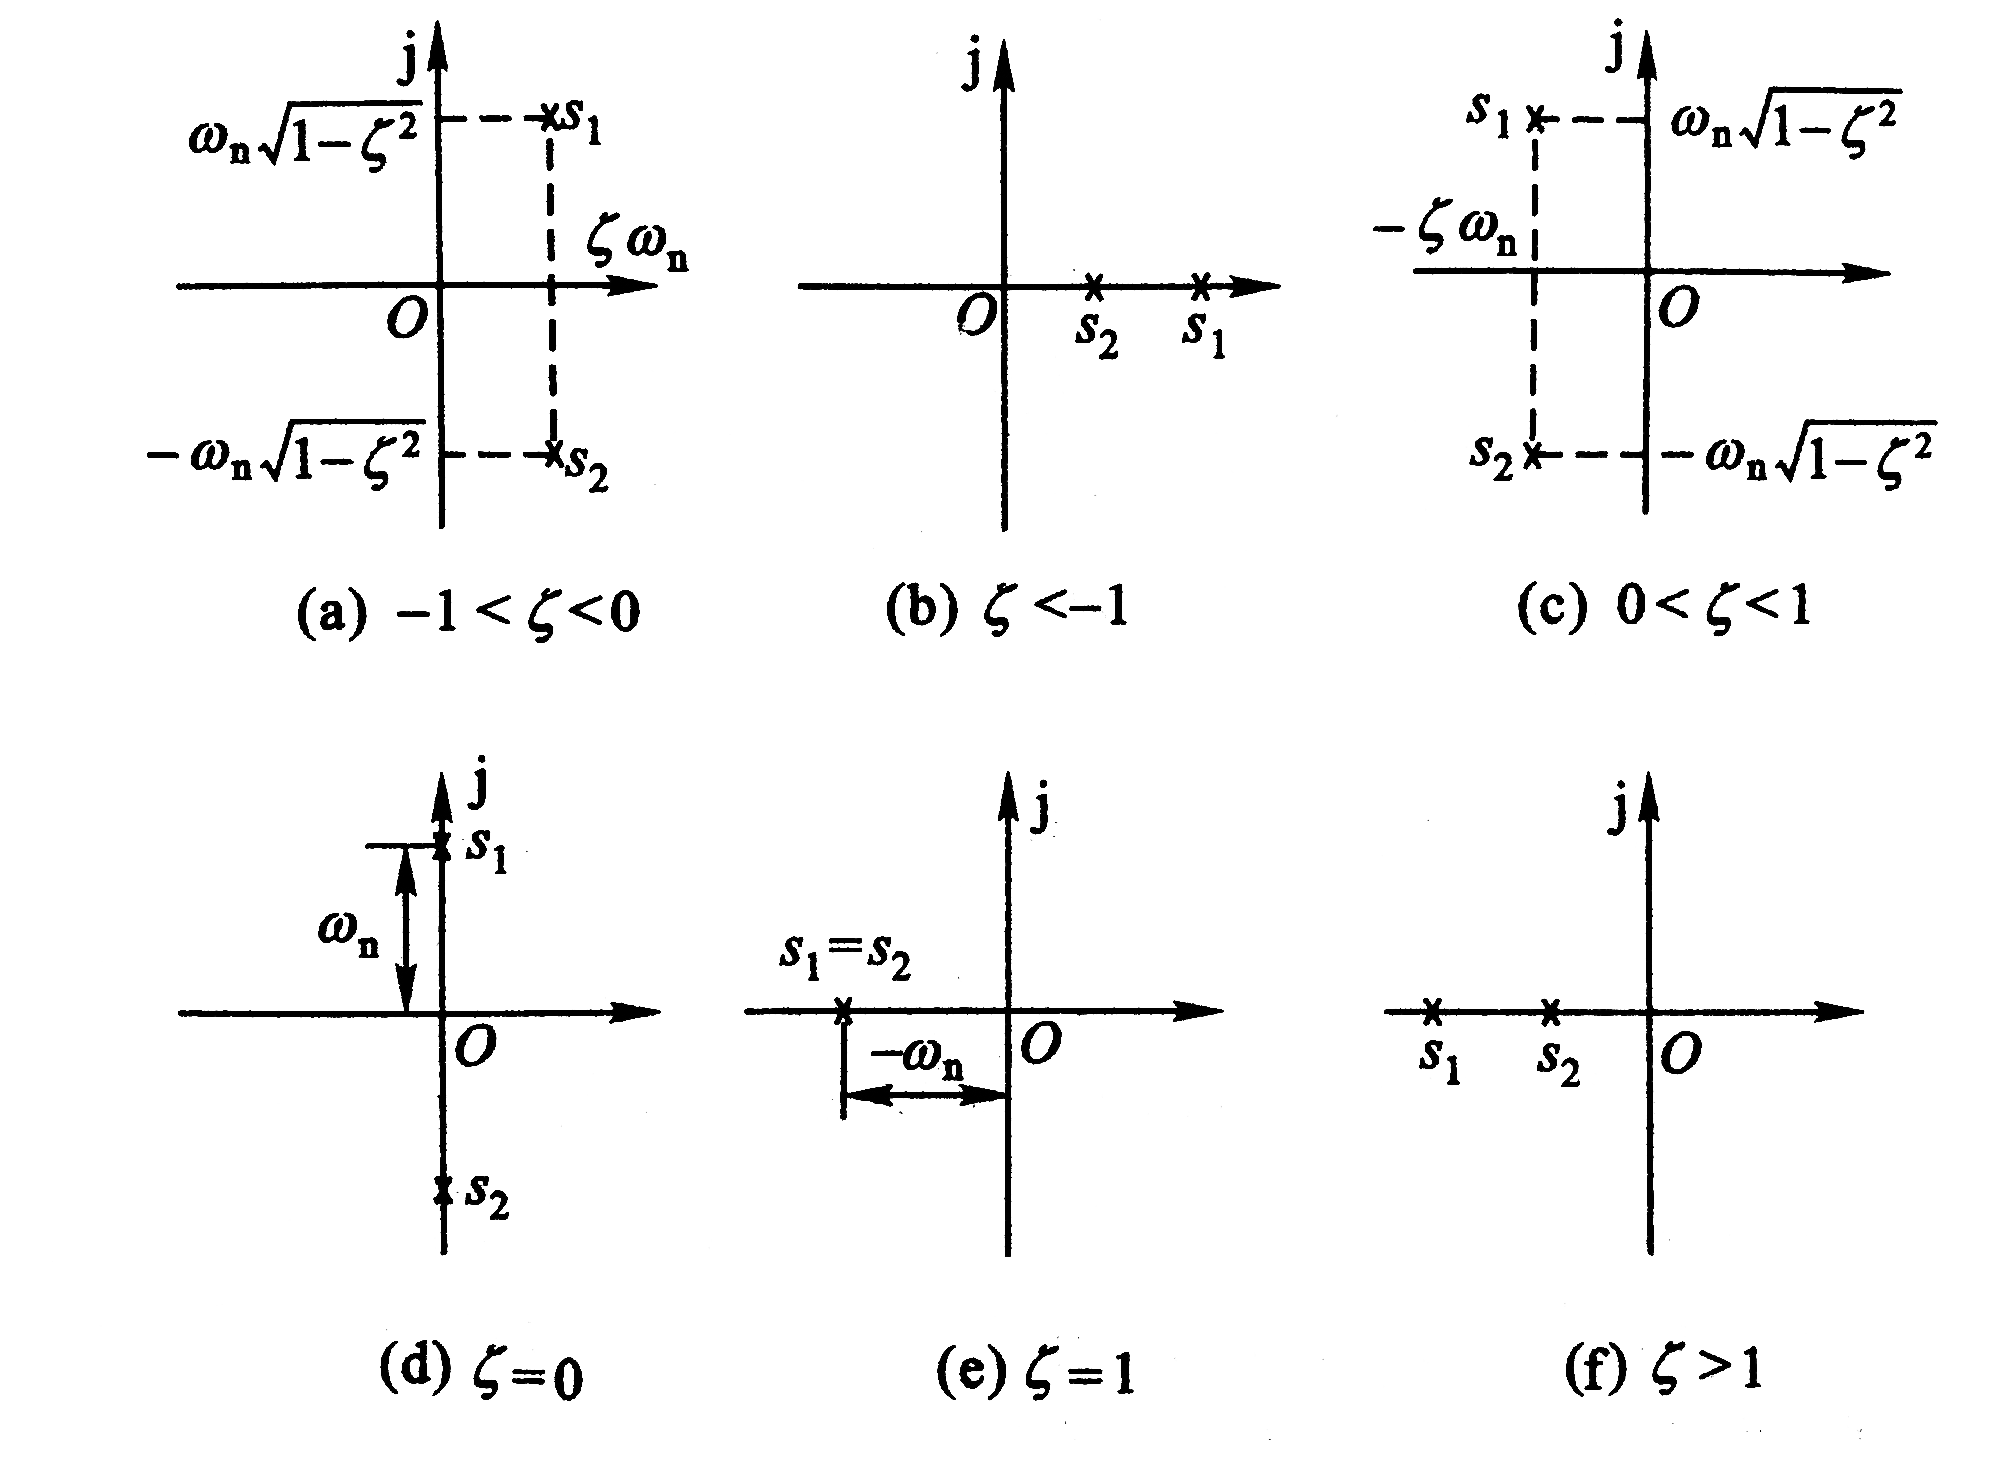
\includegraphics[width=0.7\linewidth]{pic/二阶系统.png}
		\vspace*{-0.5em}
		\captionof{figure}{$s$平面上二阶系统的闭环极点分布}
		\label{二阶系统平面}
	\end{center}
}
]

二阶系统的响应完全由$\omega_\n, \zeta$两个参数来描述,所以$\omega_\n , \zeta $是二阶系统的结构参数。对于不同的二阶系统,$\omega_\n , \zeta $的物理含义是不同的。

\vspace*{0.5em}
\subsection{二阶系统的单位跃阶响应}
\noindent \textbf{1. 过阻尼二阶系统的单位阶跃响应}
\par 当阻尼比$\zeta > 1$时,二阶系统的闭环特征方程有两个不相等的负实根。即
\begin{align}
	s^2 + 2 \zeta \omega_\n +\omega_\n^2=\left(s + \dfrac{1}{T_1}\right)\left(s + \dfrac{1}{T_2}\right)=0
\end{align}
其中,
\begin{align*}
	T_1= \dfrac{1}{\omega_\n(\zeta - \sqrt{\zeta^2 - 1})}\\
	T_1= \dfrac{1}{\omega_\n(\zeta + \sqrt{\zeta^2 - 1})}
\end{align*}
且$T_1 > T_2, \omega_\n^2 = \dfrac{1}{T_1T_2}$。传递函数为
\begin{align}
	\varPhi(s) = \dfrac{C(s)}{R(s)} = \dfrac{\dfrac{1}{T_1T_2}}{\left(s + \dfrac{1}{T_1}\right)\left(s + \dfrac{1}{T_2}\right)}=\dfrac{1}{(T_1s +1)(T_2s+1)}
\end{align}
当输入信号为单位阶跃作用时,系统的输出
\begin{align*}
	C(s) = \varPhi(s)\cdot R(s) = \dfrac{\dfrac{1}{T_1T_2}}{s \left(s + \dfrac{1}{T_1}\right)\left(s + \dfrac{1}{T_2}\right)} = \dfrac{T_2 - T_1}{s} \left(\dfrac{1}{s + \dfrac{1}{T_1}} - \dfrac{1}{s + \dfrac{1}{T_2}}\right) = \dfrac{1}{s} + \dfrac{T_1}{T_2 - T_1}\dfrac{1}{s + \dfrac{1}{T_1}} + \dfrac{T_2}{T_1 - T_2}\dfrac{1}{s + \dfrac{1}{T_2}}
\end{align*}
取Laplace逆变换,
\begin{align}
	h(t) = 1 + \dfrac{1}{\dfrac{T_2}{T_1} - 1}\e ^{- \frac{1}{T_1}t} + \dfrac{1}{\dfrac{T_1}{T_2} - 1}\e^{- \frac{1}{T_2} t}, \quad t \ge 0
\end{align}
\noindent 特点:
\begin{itemize}
	\item 曲线\\
	\hspace*{2em} 起始速度很小,然后逐渐加大到某一值后又减小,最后趋于零,因此响应曲线有一个拐点。
	\item 超调量\\
	\hspace*{2em} 过阻尼二阶系统的单位响应没有超调量。
	\item 调节时间\\
	\hspace*{2em} 没有具体的表达式,可以由计算机绘制图表如图\ref{阻尼比表}.
	常见的调节时间如下
	\begin{align*}
		\zeta = 1 \quad T_1 = T_2 \quad t_\text{s} = 4.75T_1\\
		\zeta = 1.25 \quad T_1 = 4T_2 \quad t_\text{s} = 3.3T_1\\
		\zeta > 1.25 \quad T_1 > 4 T_2 \quad t_\text{s} \approx 3 T_1
	\end{align*}
	当$T_1 > 4T_2
	$时,$\e^{-\frac{1}{T_2}t}(\zeta > 1.25)$比$\e^{-\frac{1}{T_1}t}$项衰减快很多,所以可以将系统近似看成一阶系统来计算。
	\begin{figure}[!htb]
		\centering 
		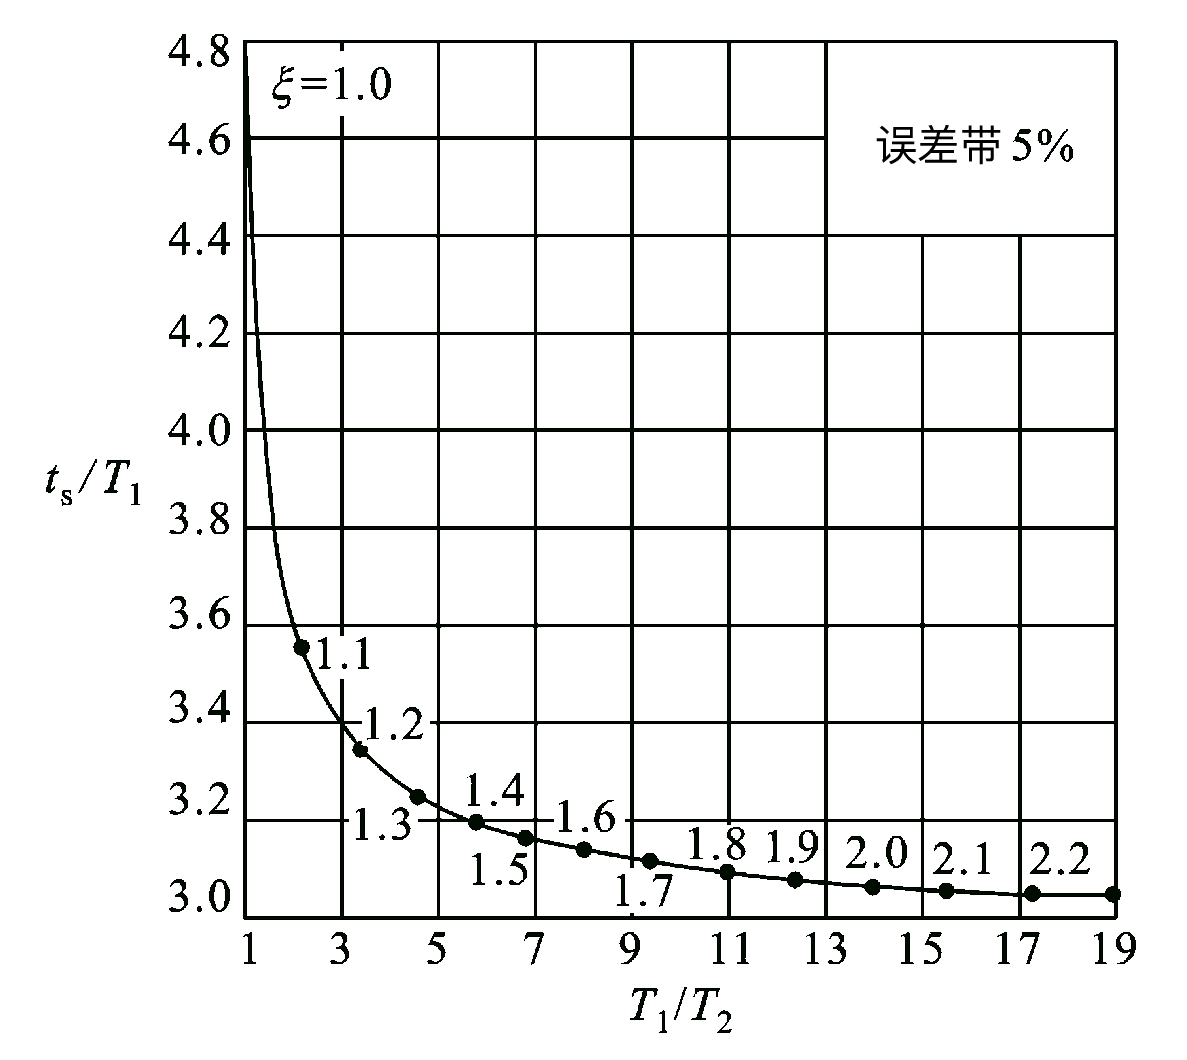
\includegraphics[width=0.5\linewidth]{pic/阻尼比表.png}
		\vspace*{-1em}
		\caption{\quad 阻尼比表}
		\label{阻尼比表}
	\end{figure}
	\item 稳态参数\\
	\hspace*{2em} 稳态参数
	\begin{align*}
		e_{\text{ss}} = 1 - h(\infty) = 1 -1 =0
	\end{align*}
\end{itemize}
 
\noindent \textbf{2. 欠阻尼二阶系统的单位阶跃响应}
\par 当$0< \zeta <1$时,得到一对共轭复根
\begin{align}
	s_{1,2} = - \zeta \omega_\n \pm \j \omega_\n \sqrt{1 - \zeta^2} = - \sigma \pm \j \omega_\text{d}
\end{align}
其中,
\begin{myitemize}
	\item $\sigma = \zeta \omega_\n$\quad 特征根实部的模值,具有角频率量纲\vspace*{-0.5em}
	\item $\omega_\text{d} = \omega_\n\sqrt{1 - \zeta^2}$ \quad \dy[阻尼振荡角频率]{ZNZDJPL}\vspace*{0.3em}
\end{myitemize}
当输入为单位阶跃信号为
\begin{align*}
	C(s) = \dfrac{\omega_\n^2}{s^2 + 2 \zeta \omega_\n s + \omega_\n^2} \cdot \dfrac{1}{s} = \dfrac{1}{s} - \dfrac{s + \zeta \omega_\n}{(s+ \zeta \omega_\n)^2 + \omega_\text{d}^2} -\dfrac{\zeta \omega_\n}{(s+ \zeta \omega_\n)^2 + \omega_\text{d}^2} 
\end{align*}
取Laplace逆变换,
\begin{align}
	h(t) &= 1 - \e^{- \zeta \omega_\n t}\left(\cos \omega_\text{d} t + \dfrac{\zeta}{\sqrt{1 - \zeta^2}\sin \omega_\text{d} t}\right)\notag\\[0.5em]
	& =1 - \dfrac{\e^{-\zeta \omega_\n t} }{\sqrt{1 - \zeta^2}}\big(\sqrt{1 - \zeta^2}\cos \omega_\text{d}t + \zeta \sin \omega_\text{d}t\big)\\[0.5em]
	& = 1 - \dfrac{\e^{-\zeta \omega_\n t}}{\sqrt{1 - \zeta^2}}\sin (\omega_\text{d}t + \beta)
	\label{欠阻尼二阶公式}
\end{align}
其中,
\begin{align}
	\beta = \arctan\left(\dfrac{\sqrt{1 - \zeta^2}}{\zeta}\right) = \arccos\zeta
\end{align}

\noindent 特点:
\begin{itemize}
	\item 曲线\\
	\hspace*{2em} 曲线的包络线为
	\begin{equation}
		1 \pm \dfrac{\e^{-\zeta \omega_n t}}{\sqrt{1 - \zeta^2}}
	\end{equation}
实际响应的收敛速度比包络线的收敛速度要快,因此往往可用包络线代替实际响应来估算调节时间。阻尼较大时,估算会带来较大误差。
	\item 上升时间\\
	\hspace*{2em}由于$h(t_\text{r})$=1,即
	\begin{align*}
		1 - \dfrac{\e^{-\zeta \omega_\n t} }{\sqrt{1 - \zeta^2}}\big(\sqrt{1 - \zeta^2}\cos \omega_\text{d}t + \zeta \sin \omega_\text{d}t\big) =  1\\[0.5em]
		\e^{-\zeta \omega_\n t} \neq 0 \Rightarrow \sqrt{1 - \zeta^2}\cos \omega_\text{d}t + \zeta \sin \omega_\text{d}t = 0\\[0.5em]
		\Rightarrow \tan \omega_\text{d} t_\text{r} = - \dfrac{\sqrt{1 - \zeta^2}}{\zeta} = \pi - \arccos \zeta
	\end{align*}
所以
\begin{align}
	t_\text{r} = \dfrac{\pi -\arccos \zeta}{\omega_\text{d}}
\end{align}
\item 峰值时间\\
\hspace*{2em}由$h'(t_\text{p}) = 0$,有
\begin{align*}
	\left. \dfrac{\d h(t)}{\d t}\right|_{t =t_\text{p}} &= (\sin \omega_\text{d} t_\text{p}) \dfrac{\omega_\n}{\sqrt{1 - \zeta^2} \e^{- \zeta \omega_\n t_\text{p}}} =0 \quad 
	\Rightarrow \quad \sin \omega_\text{d} t_\text{p} = 0\\
	&\Rightarrow \sin \omega_\text{d} t_\text{p} = 0, \pi, 2\pi , \cdots
\end{align*}
因为峰值时间对应于第一个峰值的时间,所以
\begin{align}
	 t_\text{p} = \dfrac{\pi}{\omega_\text{d}}
\end{align}
\item 超调量\\
\hspace*{2em} 将峰值时间代入二阶方程的表达式,得到最大输出量
\begin{align*}
	h(t)_{\max} = h(t_\text{p}) &= 1 - \dfrac{\e^{-\zeta \omega_\n t_\text{p}}}{\sqrt{1 - \zeta^2}}\sin (\omega_\text{d} t_\text{p} + \beta ) \\[0.5em]
	& = 1 -  \dfrac{\e^{ - \frac{\pi \zeta}{  \sqrt{1 - \zeta^{\scriptscriptstyle 2}}}}}{\sqrt{1 - \zeta^2}}\sin( \pi + \beta ) \\[0.5em]
	& = 1 +   \dfrac{\e^{ - \frac{\pi \zeta}{  \sqrt{1 - \zeta^{\scriptscriptstyle 2}}}}}{\sqrt{1 - \zeta^2}}\sin \beta \\[0.5em]
	& = 1 +   \dfrac{\e^{ - \frac{\pi \zeta}{  \sqrt{1 - \zeta^{\scriptscriptstyle 2}}}}}{\sqrt{1 - \zeta^2}}\sqrt{1 - \zeta^2} \\[0.5em]
	& = 1 + \e^{ - \frac{\pi \zeta}{  \sqrt{1 - \zeta^{\scriptscriptstyle 2}}}}
\end{align*}
所以超调量为
\begin{align}
	\sigma \, \% = \dfrac{h(t_\text{p}) - h(\infty)}{h(\infty)} = \dfrac{\e^{ - \frac{\pi \zeta}{  \sqrt{1 - \zeta^{\scriptscriptstyle 2}}}}}{1} = \e^{ - \frac{\pi \zeta}{  \sqrt{1 - \zeta^{\scriptscriptstyle 2}}}} \times 100 \,\%
\end{align}
\item 调节时间\\
\hspace*{2em} 当阻尼比$\zeta < 0.8$时,
\begin{align}
	t_\text{s} = \dfrac{3.5}{\zeta \omega_\n}\quad \mbox{(取5\%误差带)}\\[0.5em]
	t_\text{s} = \dfrac{4.5}{\zeta \omega_\n}\quad \mbox{(取2\%误差带)}
\end{align}
\item 稳定误差
\begin{align}
	e_{\text{ss}} = 1 - h(\infty) = 1- 1 = 0
\end{align}
\end{itemize}
\subsection{改善二阶系统响应的措施}

\noindent \textbf{1. 误差信号的比例-微分控制}
\begin{figure}[!htb]
	\centering
	\begin{tikzpicture}[circuit ee IEC,node distance=1.2cm]
		\node[bulb] (A)  [draw, inner sep=5pt,label=-80:$-$] {};
		\node (C) [draw, inner sep = 6pt, right of = A, node distance = 1.5cm]{$1$};
		\node[bulb] (D) [draw, inner sep = 5pt, right of = C, node distance = 1cm]{};
		\node (E) [draw, inner sep =6pt, below of = C, node distance = 1.5cm] {$T_{\text{d}}s$};
		\node (B) [draw, inner sep =4pt,right of = D, node distance = 2cm]{$\,\dfrac{\omega_\n^2}{s^2 + 2 \zeta \omega_\n s}\,$};
		
		\draw[arrows={-Stealth}] (-1cm,0cm) -- (A)node[near start, above = 0cm]{$R(s)$};
		\draw[arrows={-Stealth}] (A) --(C)node[midway, above = 0cm]{$E(s)$};
		\draw[arrows={-Stealth}] (C) -- (D);
		\draw[arrows={-Stealth}] (D) -- (B);
		\draw[arrows={-Stealth}] (0.6cm,0cm) --+ (0cm,-1.5cm) -- (E);
		\draw[arrows={-Stealth}] (E) --+ (1cm, 0cm) -- (D);
		\draw[arrows={-Stealth}] (B) --+(2cm,0cm)node[near end, above= 0cm]{$C(s)$};
		\draw[arrows={-Stealth}] (6cm, 0cm) -- (6cm, -2.3cm) -- (0cm, -2.3cm) -- (A);
		 
	
	\end{tikzpicture}
	\caption{比例—微分控制的二阶系统结构图}
	\label{比例微分控制的二阶系统}
\end{figure}

\noindent 图\ref{比例微分控制的二阶系统}.为一个具有比例—微分控制的二阶系统的结构图。其中,$T_\text{d}$表示微分时间常数。系统的参数如下:
\begin{itemize}
	\item 系统的开环传递函数
	\begin{align}
		G(s) = \dfrac{C(s)}{E(s)} = \dfrac{\omega_n^2(1+ T_{\text{d}}s)}{s^2+2\zeta \omega_ns}
	\end{align}
	\item 系统的闭环传递函数
	\begin{align}
		\varPhi(s) = \dfrac{C(s)}{R(s)} =  \dfrac{\omega_n^2(1+ T_{\text{d}}s)}{s^2+(2\zeta \omega_n + T_{\text{d}}\omega_n^2)s+\omega_n^2}
	\end{align}
	\item 等效阻尼比
	\begin{align}
		\zeta_{\text{d}} = \zeta +\dfrac{1}{2}T_{\text{d}}\omega_n
	\end{align}
\end{itemize}

引入比例-微分控制使系统的等效阻尼比增加,从而抑制了振荡,使超调减弱,可改善系统的平稳性。

微分作用之所以能改善动态性能,因为它产生一种早期控制(或称为超前控制),能在实际超调量出来之前,就产生一个修正作用。

由等效图\ref{比例微分控制的二阶系统等效图},可以得到
\begin{align*}
	c(t) = c_1(t) + c_2(t)
\end{align*}
\noindent $c(t),c_1(t),c_2(t)$的图像大致如图\ref{ct}.
\vspace*{2em}

\noindent 比例微分环节的作用如下:
\begin{itemize}
	\item 一方面,增加$T_\text{d}$项,增大了等效阻尼比$\zeta_{\text{d}}$,使$c_1(t)$曲线比较平稳。
	\item 另一方面,它又使$c_1(t)$加上了它的微分信号$c_2(t)$ ,加速了$c(t)$的响应速度,但也同时削弱了等效阻尼比$\zeta_{\text{d}}$的平稳作用。\vspace*{1em}
\end{itemize}

\begin{figure}[!htb]
	\centering
	\begin{tikzpicture}[circuit ee IEC,node distance=1.2cm]
		\node (A) [draw, inner sep =6pt]{$\dfrac{\omega_n^2}{s^2+(2\zeta \omega_n + T_{\text{d}}\omega_n^2)s+\omega_n^2}$};
		\node (B) [draw, inner sep =6pt, above of = A, node distance =1.5cm, xshift = 4cm]{$\,\,1\,\,$};
		\node (C) [draw, inner sep = 6pt, below of = B, node distance =3cm]{$T_{\text{d}} s$};
		\node[bulb] (D) [draw, inner sep =5pt, right of = A, node distance = 5.5cm]{};
		
		\draw[arrows={-Stealth}] (-3.5cm, 0cm) -- (A)node[near start, above = 0cm]{$R(s)$};
		\draw[arrows={-Stealth}] (A) --+ (2.5cm,0cm) --+(2.5cm, 1.5cm) -- (B);
		\draw[arrows={-Stealth}] (B) --+ (1.5cm,0cm) --+(D)node[near start, above=0cm,xshift = 5mm,yshift = 2mm]{$C_1(s)$}; 
		\draw[arrows={-Stealth}] (A) --+ (2.5cm,0cm) --+(2.5cm, -1.5cm) -- (C);
		\draw[arrows={-Stealth}] (C) --+ (1.5cm,0cm) --+(D)node[near start, above=0cm,xshift = 5mm,yshift = -2mm]{$C_2(s)$}; 
		\draw[arrows={-Stealth}] (D) --+ (1.5cm,0cm)node[near end, above=0cm]{$C(s)$}; 
		
	\end{tikzpicture}
	\caption{比例—微分控制的二阶系统结构等效图}
	\label{比例微分控制的二阶系统等效图}
\end{figure}

\begin{figure}[!htb]
	\centering
	\includegraphics[width=0.65\linewidth]{pic/ct图.png}
	\caption{$c_1(t),c_2(t),c(t)$曲线}
	\label{ct}
\end{figure}

\noindent \textbf{2. 测速反馈}

如图\ref{测速反馈控制的二阶系统},测速反馈可以改善系统品质
\begin{figure}[!htb]
	\centering
	\begin{tikzpicture}[circuit ee IEC,node distance=1.2cm]
		\node[bulb] (A) [draw, inner sep = 5pt, label=-85:$-$]{};
		\node[bulb] (B) [draw, right of = A, node distance = 1.5cm,inner sep = 5pt, label=-85:$-$]{};
		\node (C) [draw, inner sep =6pt, right of = B,node distance =2cm]{$\dfrac{K}{Js+B}$};
		 \node (D) [draw, inner sep =6pt, right of = C,node distance = 2.5cm]{$\dfrac{1}{s}$};
		 \node (E) [draw, inner sep = 6pt, below of = C, node distance = 1.6cm]{$K_h$};
		 
		 \draw[arrows={-Stealth}] (-1cm,0cm) -- (A)node[near start, above = 0cm]{$\theta_r$};
		 \draw[arrows={-Stealth}] (A) -- (B);
		 \draw[arrows={-Stealth}] (B) -- (C);
		 \draw[arrows={-Stealth}] (C) -- (D)node[midway, above = 0cm]{$\dot{\theta}_m$};
		 \draw[arrows={-Stealth}] (D) -- +(1.5cm,0cm)node[near end,above = 0cm]{$\theta_m$};
		 \draw[arrows={-Stealth}] (5cm, 0cm) --+(0cm,-1.6cm) -- (E);
		 \draw[arrows={-Stealth}] (E) --+ (-2cm,0cm) -- (B);
		 \draw[arrows={-Stealth}] (6.75cm, 0cm) -- +(0cm,-2.5cm) -- (0cm, -2.5cm) -- (A);
	\end{tikzpicture}
\caption{测速反馈控制的二阶系统}
\label{测速反馈控制的二阶系统}
\end{figure}

\begin{figure}[!htb]
	\centering
	\begin{tikzpicture}[circuit ee IEC,node distance=1.2cm]
		\node[bulb] (A) [draw, inner sep = 5pt, label=-85:$-$]{};
		\node[bulb] (B) [draw, right of = A, node distance = 1.5cm,inner sep = 5pt, label=-85:$-$]{};
		\node (C) [draw, inner sep =6pt, right of = B,node distance =2cm]{$\dfrac{K}{Js+B}$};
		\node (D) [draw, inner sep =6pt, right of = C,node distance = 2.5cm]{$\dfrac{1}{s}$};
		\node (E) [draw, inner sep = 6pt, below of = C, node distance = 1.6cm]{$K_h s$};
		
		\draw[arrows={-Stealth}] (-1cm,0cm) -- (A)node[near start, above = 0cm]{$\theta_r$};
		\draw[arrows={-Stealth}] (A) -- (B);
		\draw[arrows={-Stealth}] (B) -- (C);
		\draw[arrows={-Stealth}] (C) -- (D)node[midway, above = 0cm]{$\dot{\theta}_m$};
		\draw[arrows={-Stealth}] (D) -- +(1.5cm,0cm)node[near end,above = 0cm]{$\theta_m$};
		\draw[arrows={-Stealth}] (6.75cm, -1.6cm)  -- (E);
		\draw[arrows={-Stealth}] (E) --+ (-2cm,0cm) -- (B);
		\draw[arrows={-Stealth}] (6.75cm, 0cm) -- +(0cm,-2.5cm) -- (0cm, -2.5cm) -- (A);
	\end{tikzpicture}
\caption{测速反馈控制的二阶系统等效图}
\label{测速反馈控制的二阶系统等效图}
\end{figure}
\noindent 在数学上等效于图\ref{测速反馈控制的二阶系统等效图}.
\begin{itemize}
	\item 无测速反馈时$K_h = 0$
	\begin{align}
		\dfrac{\Theta_m(s)}{\Theta_r(s)} = \dfrac{K/J}{s^2 + (B/J)s + K/J} = \dfrac{\omega_n^2}{s^2 + 2 \zeta \omega_n s + \omega_n^2}
	\end{align}
其中\vspace*{-1em}
\begin{itemize}
	\item $\omega_n = \sqrt{K/J}$
	\item $\zeta = \dfrac{B}{2 \sqrt{KJ}}$
\end{itemize}
	\item 有测速反馈时
	\begin{align}
		\dfrac{\Theta_m(s)}{\Theta_r(s)} =  \dfrac{\omega_n^2}{s^2 + 2 (\zeta + K_h\omega_n/2) \omega_n s + \omega_n^2}
	\end{align}
阻尼比变为
\begin{align}
	\zeta_t = \zeta + \dfrac{1}{2} K_h \omega_n
\end{align}
\end{itemize}


\noindent \textbf{3. 比例-微分控制和速度反馈控制比较}
\begin{enumerate}[\hspace*{2em}(1)]
	\item 比例-微分控制的线路结构比较简单,成本低,而速度反馈控制部件则较昂贵。
	\item 从抗干扰来看,前者抗干扰能力较后者差。
	\item 两者均能改善系统的平稳性。在相同的阻尼比和自然频率下,采用速度反馈不足之处是其会使系统的开环增益下降,但却能使内回路中被包围部件的非线性特性、参数漂移等不利影响大大削弱。
\end{enumerate}


\section{一二阶系统总结}
\noindent \textbf{1. 一阶系统}
\begin{myitemize}
	\item 传递函数$\displaystyle \varPhi(s) = \dfrac{1}{Ts + 1}$
	\item 单位阶跃输出$h(t) = 1 - \e^{- \frac{1}{T} t}$
	\item 调节时间
	$t_{\text{s}} = \begin{cases}
		3T, \quad \mbox{对应5 \%误差带}\\
		4T, \quad \mbox{对应2 \%误差带}
	\end{cases}$
	\item 超调量$\sigma \,\% = 0$
	\item 稳态误差$e_{\text{ss}} = 1 - h(\infty) = 0$\vspace*{0.3em}
\end{myitemize}
\vspace*{0.5em}
\noindent \textbf{2. 二阶系统}
\begin{myitemize}
	\item 传递函数$\displaystyle \varPhi(s) = \dfrac{\omega_\n^2}{s^2 + 2 \zeta \omega_\n s + \omega_n^2}$
	\item 特征方程$s^2 + 2\zeta \omega_\n s +\omega_\n^2 = 0$
	\vspace*{0.3em}
\end{myitemize}
\begin{itemize}
	\item 过阻尼$\zeta > 1$
	
	\begin{myitemize}
		\item 单位阶跃输出$h(t) = 1 + \dfrac{1}{\dfrac{T_2}{T_1} - 1}\e ^{- \frac{1}{T_1}t} + \dfrac{1}{\dfrac{T_1}{T_2} - 1}\e^{- \frac{1}{T_2} t}, \quad t \ge 0$
		\item 调节时间$t_\text{s}$无固定表达式,见图\ref{阻尼比表}.常见的调节时间为
		$\begin{aligned}
			&\zeta = 1 \quad T_1 = T_2 \quad t_\text{s} = 4.75T_1\\
			&\zeta = 1.25 \quad T_1 = 4 T_2 \quad t_\text{s} = 3.3T_1\\
			&\zeta > 1.25 \quad T_1 > 4 T_2 \quad t_\text{s} \approx 3 T_1
		\end{aligned}$
	\item 超调量$\sigma \, \% = 0$
	\item 稳态参数$e_\text{ss} = 0$\vspace*{0.5em}
	\end{myitemize}

	\item 欠阻尼$0 < \zeta < 1$
	
\begin{myitemize}
	\item 单位阶跃输出$ h(t) = 1 - \dfrac{\e^{-\zeta \omega_\n t}}{\sqrt{1 - \zeta^2}}\sin (\omega_\text{d}t + \beta), \quad \omega_\text{d} = \omega_\n \sqrt{1 - \zeta^2}, \beta = \arccos\zeta$
	\item 上升时间$t_\text{r} = \dfrac{\pi - \beta}{\omega_\text{d}} $
	\item 峰值时间$t_\text{p} = \dfrac{\pi}{\omega_\text{d}}$
	\item 调节时间 $\begin{aligned}
		t_\text{s} = \dfrac{3.5}{\zeta \omega_\n} \,\,\mbox{取5\%误差带}\\
		t_\text{s} = \dfrac{4.5}{\zeta \omega_\n} \,\,\mbox{取2\%误差带}\\
	\end{aligned}\quad \zeta < 0.8$
	\item 超调量$\sigma \, \% = \e^{ - \frac{\pi \zeta}{  \sqrt{1 - \zeta^{\scriptscriptstyle 2}}}} \times 100 \,\%$
	\item 稳态参数$e_\text{ss} = 0$\vspace*{0.5em}
\end{myitemize}
\end{itemize}



\section{系统稳定性分析}
\subsection{系统稳定性概念}
\tdefination[系统稳定性]
如果一个控制系统收到扰动,偏离了原来的平衡状态,产生偏差,而当扰动消失之后,系统又能够逐渐恢复到原来的平衡状态,则称系统是稳定的,或具有\dy[稳定性]{WDX}。

稳定性是系统自身的一种恢复能力,是系统的一种固有属性。对于现在讨论的定常系统来说,这种固有的稳定性只取决于系统的结构、参数,而与初始条件及外作用无关。\vspace*{1em}

\subsection{稳定的数学条件}
设系统的线性化增量方程为
\begin{align}
	a_0 \dfrac{\d^n c(t)}{\d t} + a_1 \dfrac{\d^{n-1} c(t)}{\d t^{n-1}}+\cdots + a_{n-1}\dfrac{\d c(t)}{\d t} + a_nc(t) = b_0\dfrac{\d^m r(t)}{\d t^m} + b_1 \dfrac{\d^{m-1} r(t)}{\d t^{m-1}} + \cdots + b_{m-1}\dfrac{\d r(t)}{\d t} + b_mr(t)
	\label{WDX1}
\end{align}
其特征方程为
\begin{align}
	D(s) = a_0s^n + a_1 s^{n-1} + \cdots + a_{n-1}s +a_n=0
\end{align}
假设特征方程$D(s) = 0$有$n$个互异的特征根$s_i$,则
\begin{align}
	D(s) = a_0 \prod_{i = 1}^{n}(s - s_i)
\end{align}
作反变换可得微分方程\ref{WDX1}的解为
\begin{align}
	c(t) = \sum_{i = 1}^{n}A_i\e^{s_i t}+c^*(t)
\end{align}
其中,
\begin{myitemize}
	\item $\displaystyle  \sum_{i = 1}^{n}A_i\e^{s_i t}$是微分方程的通解,取决于特征根$s_i$,即由系统的结构参数决定
	\item $\displaystyle c^*(t)$是微分方程的特解,其运动规律取决于输入作用
\end{myitemize}
所以,系统稳定等价于
\begin{align}
	\lim\limits_{t \to \infty}  \sum_{i = 1}^{n}A_i\e^{s_i t} = 0
\end{align}
即
\begin{align}
	\lim\limits_{t \to \infty}  \sum_{i = 1}^{n}\e^{s_i t} = 0
\end{align}

\theorem[系统稳定的充要条件]
\begin{myitemize}
	\item 所有特征根都具有负实部$\Longleftrightarrow$ 系统稳定
	\item 任意一个特征根实部为正$\Longrightarrow$ 系统发散
	\item 存在特征根部分为0的单根,其余均有负实部$\Longrightarrow$ 系统处于临界状态,既不发散也不能恢复原来的状态
	\item 实部为重根$\Longrightarrow$ 系统发散\vspace*{0.3em}
\end{myitemize}

\subsection{系统稳定性判据}
\ttheorem[赫尔维茨(Hurwitz)判据]
系统特征根方程的一般形式为\index{HEWZ@赫尔维茨判据}
\begin{align*}
	D(s) = a_0 s^n + a_1 s^{n-1} + \cdots + a_{n-1}s + a_n =0
\end{align*}
假设首项系数$a_0>0$.

系统稳定的充要条件:特征方程的\dy[赫尔维茨行列式]{HEWCHLS}$D_k(k = 1,2,3,\cdots,n)$全部为正。各阶赫尔维茨行列式为
\begin{align}
	D_1 &= a_1, \notag \\
	D_2 &= 
	\begin{vmatrix}
		\,\, a_1 & a_3 \,\,\\
		\,\, a_0 & a_2 \,\,
	\end{vmatrix},\notag \\
	D_3 &= 
	\begin{vmatrix}
		\mjg a_1 & a_3 & a_5\mjg\\
		\mjg a_0 & a_2 & a_4\mjg\\
		\mjg 0 & a_1 & a_3 \mjg
	\end{vmatrix},\notag\\
	\cdots \notag \\
D_n &= 
\begin{vmatrix}
	\mjg a_1 & a_3 & a_5 & \cdots & a_{2n-1}\mjg\\
	\mjg a_0 & a_2 & a_4 & \cdots & a_{2n-2}\mjg\\
	\mjg 0 & a_1 & a_3 & \cdots & a_{2n-3}\mjg\\
	\mjg 0 & a_0 & a_2 & \cdots & a_{2n-4}\mjg\\
	\mjg \vdots & \vdots & \vdots & & \vdots\mjg\\
	\mjg 0 & 0 & 0& \cdots & a_n\mjg
\end{vmatrix}
\end{align}

\examples 系统的特征方程为
\begin{align*}
	a_0 s^3 + a_1 s^2 + a_2 s + a_3 = 0 \quad (a_0 >0)
\end{align*}
判别系统的稳定性。
\newpage

\vspace*{-2em}
\solve 系统稳定的充要条件为
\begin{align*}
	D_1  = a_1 >0, \quad 
	D_2  = 
	\begin{vmatrix}
		\,\, a_1 & a_3 \,\,\\
		\,\, a_0 & a_2 \,\,
	\end{vmatrix}
= a_1 a_2 -a_0a_3 >0
\end{align*}
\vspace*{-1.5em}
\begin{align*}
D_3  = 
\begin{vmatrix}
	\mjg a_1 & a_3 & a_5\mjg\\
	\mjg a_0 & a_2 & a_4\mjg\\
	\mjg 0 & a_1 & a_3 \mjg
\end{vmatrix}
 = a_1a_2a_3 - a_0a_3^2 >0
\end{align*}

\theorem[林纳德-奇帕特(Lienard-Chipard)判据]
系统稳定的充要条件是:\index{LND@林纳德-奇帕特}
\begin{myitemize}
	\item 系统特征方程的各项系数大于0,即$a_i>0,(i = 0,1,2,\cdots,n)$\vspace*{-0.8em}
	\item 奇数阶或偶数阶的赫尔维茨行列式大于0,即$D_{\mbox{\scriptsize 奇}}>0$或$D_{\mbox{\scriptsize 偶}}>0$\vspace*{0.3em}
\end{myitemize}
\warn[
\hspace*{2em}$a_i > 0$是系统稳定的必要条件,即$a_i > 0 $不满足,则系统一定不稳定。当$a_i>0$满足时,需要计算半数的赫尔维茨行列式才能进一步判断系统是否稳定。
]

\examples 系统特征方程为
\begin{align*}
	a_0 s^3 + a_1 s^2 + a_2 s + a_3 = 0 \quad (a_0 >0)
\end{align*}
判别系统的稳定性。

\solve 系统稳定的充要条件为
\begin{align*}
	a_0>0,a_1>0,a_2>0,a_3>0\\
	D_2  = 
\begin{vmatrix}
	\, a_1 & a_3 \,\,\\
	\, a_0 & a_2 \,\,
\end{vmatrix}
= a_1 a_2 -a_0a_3 >0
\end{align*}
\vspace*{1em}

\theorem[劳斯(Routh)判据]
若系统的特征方程为\index{LXBH@劳斯判据}
\begin{align*}
	D(s) = a_0s^n + a_1 s^{n-1} + \cdots + a_{n-1}s + a_n = 0
\end{align*}
系统稳定的充分必要条件是劳斯表中第一列所以元素符号相同(但不为0)。\textbf{若系统不稳定,劳斯表第一列元素必有改变,改变的次数等于特征方程中正实数根的数目。}

\begin{table}[!htb]
	\centering
	\setlength{\tabcolsep}{6mm}{
		\begin{tabular}{c|c|c|c|c|c}
			\hline
			$s^n$ & $a_0$ & $a_2$ & $a_4$ & $a_6$ & $\cdots $ \\
			\hline
			$s^{n-1}$ & $a_1$ & $a_3$ & $a_5$ & $a_7$ & $\cdots$ \\
			\hline 
			& & & & & \vspace*{-1.2em}\\
			$s^{n-2}$ & $c_{13} = \dfrac{a_1a_2 - a_0a_3}{a_1}$ & $c_{23} = \dfrac{a_1a_4 - a_0a_5}{a_1}$ & $c_{33} = \dfrac{a_1a_6 - a_0a_7}{a_1}$ & $c_{43}$ & $\cdots$\\
			& & & & & \vspace*{-1.2em}\\
			\hline
			& & & & & \vspace*{-1.2em}\\
			$s^{n-3}$ & $c_{14} = \dfrac{c_{13}a_3 - a_1c_{23}}{c_{13}}$ & $c_{24} =  \dfrac{c_{13}a_5 - a_1c_{33}}{c_{13}}$ & $c_{34} =  \dfrac{c_{13}a_7 - a_1c_{23}}{c_{13}}$ & $c_{44}$ & $\cdots$\\
			& & & & & \vspace*{-1.2em}\\
			\hline
			& & & & & \vspace*{-1.2em}\\
			$s^{n-4}$ & $c_{15} = \dfrac{c_{14}c_{23} - c_{13}c_{24}}{c_{14}}$ & $c_{25} =  \dfrac{c_{14}c_{33} - c_{13}c_{34}}{c_{14}}$ & $c_{35} =  \dfrac{c_{14}c_{43} - c_{13}c_{44}}{c_{14}}$ & $c_{45}$ & $\cdots$\\
			& & & & & \vspace*{-1.2em}\\
			\hline
			$\vdots$ & $\vdots$ & $\vdots$ & $\vdots$ & $\vdots$ & $\vdots$ \\ 
			\hline
			$s^2$ & $c_{1,n-1}$ & $c_{2,n-1}$ & &&\\
			\hline
			$s^1$ & $c_{1,n}$ &&&&\\
			\hline
			$s^0$ & $c_{1,n+1} = a_n$ &&&&\\
			\hline
		\end{tabular}
}
\caption{劳斯表}
\label{劳斯表}
\end{table}

我们可以得到\textbf{(劳斯表的系数$i = 1, 2, 3, \cdots$为列数,$j = 1, 2, 3, \cdots, n+1$为行数)}
\begin{align}
	c_{i,j} = 
	\begin{cases}
		a_{2i - 2} &j=1\\
		a_{2i - 1} & j =2\\
		-\dfrac{1}{c_{1,j-1}}
		\begin{vmatrix}
			\,\, c_{1,j-2} & c_{i+1,j-2} \,\,\\
			\,\, c_{1,j-1} & c_{i+1,j-1} \,\,
		\end{vmatrix} &3<j<n\\
	a_n & j = n+1
	\end{cases}
\end{align}
\vspace*{2em}

\noindent \textbf{劳斯表判据的特殊情况}\quad 下列情形需要对劳斯判据进行修正。
\begin{itemize}
	\item 第一列某个元素为零,但该行其它元素不全为零
	\begin{myitemize}
		\item 此时,将零元素用非常小的正数$\varepsilon$代替即可
		\vspace*{0.3em}
	\end{myitemize}

\examples $D(s) = s^5+2s^4 + 2s^3 + 4s^2 +11s+10$的劳斯表如下
\begin{center}
	\begin{tabular}{cccc}
		$s^5$ & 1 & 2 & 11 \\
		$s^4$ & 2 &4 & 10 \\
		$s^3$ & $0 \approx \varepsilon$ &6 &\\
		$s^2$ & $c_1$ &&\\
		$s^1$ & $d_1$ &&\\
		$s^0$ & 10 &&\\
	\end{tabular}
\end{center}
其中,$\varepsilon \to 0 $,即
\begin{align}
	c_1 &= \dfrac{4 \varepsilon - 12}{\varepsilon} < 0\\
	d_1 &= \dfrac{6 c_1 - 10\varepsilon}{c_1} \to 6 >0 
\end{align}
所以,第一列有两次变号,有两个根在右半平面。
	\item 某行的元素全为零
	\begin{myitemize}
		\item 如果劳斯表中出现全零行,表面特征方程中存在一些大小相等,但位置相反的根。\vspace*{-1em}
		\item 这时,可以用全零行上一行的系数构造一个辅助方程,对其求导\vspace*{-1em}
		\item 用所得方程的系数代替全零行,然后继续按劳斯表的运算规则继续运算\vspace*{0.3em}
	\end{myitemize}

\examples $D(s) = s^6 + s^5 -2s^4 -3s^3 - 7s^2 -4s -4 = 0$的劳斯表如下
\begin{center}
	\begin{tabular}{ccccc}
		$s^6$ & 1 & $-2$ & $-7$ & $-4$ \\
		$s^5$ & 1 &$-3$ & $-4$ & \\
		$s^4$ & 1 &$-3$ & $-4$ & \\
		$s^3$ & 0 & 0 &  &\\
	\end{tabular}
\end{center}
由于出现全零行,构造辅助函数:$F(s) = s^4 - 3s^2 -4 = 0$,对其求导数,得
\[
\dfrac{\d F(s)}{\d s} = 4s^3 - 6s = 0
\]
将系数替换原来的零行,继续运算得
\begin{center}
	\begin{tabular}{ccccc}
		$s^6$ & 1 & $-2$ & $-7$ & $-4$ \\
		$s^5$ & 1 &$-3$ & $-4$ & \\
		$s^4$ & 1 &$-3$ & $-4$ & \\
		$s^3$ & 4& $-6$ &  &\\
		$s^2$ & $-$1.5 & $-$4 &  &\\
		$s^1$ & $-$16.7 & 0 &&\\
		$s^0$ & $-$4 &&&\\ 
	\end{tabular}
\end{center}
所以,第一列有一次变号,有一个正实部根。
\end{itemize}


\subsection{相对稳定性分析}
\tdefination[稳定度]
为了保证系统有一定稳定裕度,且具有良好度动态性能,希望特征根$s$左半平面且与虚轴有一定距离,通常称为\dy[稳定度]{WDD}。\vspace*{1em}

\noindent 计算系统度稳定度的方法如下:
\begin{enumerate}
	\item 构造新的变量$s_1 = s + a \Rightarrow s = s_1 - a$
	\item 代入原来的系统特征方程,得到新的特征方程
	\item 利用劳斯判据判断新特征方程是否稳定
\end{enumerate}

\subsection{结构不稳定及改进措施}
某些系统,仅靠调整参数仍无法稳定,称为\dy[结构不稳定系统]{JGBWDXT},例如液位控制系统
\begin{figure}[!htb]
	\centering
	\centering
	\begin{tikzpicture}[circuit ee IEC]
		\node(A) [draw, inner sep =6pt]{$K_{\text{p}}$};
		\node(E) [draw, inner sep =6pt, right of = A, node distance = 2cm]{$\dfrac{K_{\text{m}}}{s(T_{\text{m}s + 1})}$};
		\node(F) [draw, inner sep =6pt, right of = E, node distance = 2cm]{$K_1$};
		\node[bulb] (C) [draw, inner sep = 5pt, right of = F, node distance = 1.5cm, label = 95:$-$] {};
		\node (D) [draw, inner sep = 6pt, right of = C, node distance = 1.5cm]{$\dfrac{K_0}{s}$};
		\node[bulb] (O) [draw, inner sep =5pt, left of = A, node distance = 1.5cm, label = -95:$-$]{};
		
		\draw[arrows={-Stealth}](-3cm, 0) -- (O)node[near start, above = 0mm]{$H_0$} -- (A) -- (E) -- (F) -- (C) -- (D) -- +(1.5cm, 0cm)node[midway, above = 0mm,xshift = 5mm]{$H$};
		\draw[arrows={-Stealth}](8cm, 0cm) -- +(0cm, -1.5cm)  -- (-1.5cm,-1.5cm) -- (O);
		\draw[arrows={-Stealth}](5.5cm, 1.5cm) -- (C)node[near start, xshift = 0.5cm]{$Q_1$};
	\end{tikzpicture}
	\caption{液位控制系统的系统结构图}
\end{figure}

其系统闭环特征方程为
\begin{align*}
	T_{\text{m}}s^3 + s^2 + K = 0
\end{align*}
其中,$K = K_\text{p}K_{\text{m}}K_1K_0$

可以看出,系数缺项,显然不满足系统稳定的必要条件,且无论怎么调整系统参数,都不能使系统稳定。消除结构不稳定的措施有两种:
\begin{itemize}
	\item 改变积分性质
	\item 引入比例-微分控制,补上特征方程中的缺项
\end{itemize}
\noindent \textbf{1. 改变积分性质}

用反馈$K_H$包围积分环节或者包围电动机的传递函数,破坏其积分性质。
	\begin{figure}[!htb]
		\begin{center}
		\begin{minipage}{0.38\linewidth}
		\begin{tikzpicture}[circuit ee IEC]
			\node[bulb] (A) [draw, inner sep =5pt]{};
			\node (B) [draw, inner sep =6pt, right of = A, node distance =1.5cm]{$\dfrac{K_0}{s}$};
			\node (C) [draw, inner sep =6pt, below of = B, node distance =1.5cm]{$K_\text{H}$}; 
			
			\draw[arrows={-Stealth}] (-1cm, 0cm)node[xshift = -1cm]{} -- (A)node[near start, above = 0cm]{$X_1$};
			\draw[arrows={-Stealth}] (A) -- (B);
			\draw[arrows={-Stealth}] (B) -- +(2cm,0cm)node[near end, above = 0cm]{$X_2$};
			\draw[arrows={-Stealth}] (3cm, 0cm) -- (3cm, -1.5cm) -- (C);
			\draw[arrows={-Stealth}] (C) -- +(-1.5cm,0cm) -- (A);
			
		\end{tikzpicture}
	\end{minipage}
	\begin{minipage}{0.4\linewidth}
		\begin{tikzpicture}[circuit ee IEC]
			\node[bulb] (A) [draw, inner sep =5pt]{};
			\node (B) [draw, inner sep =6pt, right of = A, node distance =1.5cm,]{$\dfrac{K_\text{m}}{s(T_\text{m} s + 1)}$};
			\node (C) [draw, inner sep =6pt, below of = B, node distance =1.5cm]{$K_\text{H}$}; 
			
			\draw[arrows={-Stealth}] (-1cm, 0cm) -- (A)node[near start, above = 0cm]{$X_1$};
			\draw[arrows={-Stealth}] (A) -- (B);
			\draw[arrows={-Stealth}] (B) -- +(2cm,0cm)node[near end, above = 0cm]{$X_2$};
			\draw[arrows={-Stealth}] (3cm, 0cm) -- (3cm, -1.5cm) -- (C);
			\draw[arrows={-Stealth}] (C) -- +(-1.5cm,0cm) -- (A);
		\end{tikzpicture}
	\end{minipage}
\end{center}
\end{figure}
\begin{align*}
	\dfrac{X_2(s)}{X_1(s)} = \dfrac{K_0}{s+K_0K_\text{H}}  \hspace*{7em} \dfrac{X_2(s)}{X_1(s)} = \dfrac{K_\text{m}}{(T_\text{m}s + 1)+K_\text{m}K_\text{h}}
\end{align*}

\noindent \textbf{2. 引入比例-微分控制}

在原系统的前向通路中引入比例-微分控制:
\begin{figure}[!htb]
	\centering
	\begin{tikzpicture}[circuit ee IEC]
		\node [bulb] (A) [draw,inner sep =5pt, label=-85:$-$]{};
		\node (B) [draw, inner sep =6 pt, right of = A, node distance =1.5cm]{$\tau s + 1$};
		\node (C) [draw, inner sep =6 pt, right of = B, node distance =2.5cm]{$\dfrac{K}{s^2 (T_\text{m}s + 1)}$};
		
		\draw[arrows={-Stealth}] (-1cm,0cm) -- (A)node[near start, above = 0cm]{$H_0(s)$};
		\draw[arrows={-Stealth}] (A) -- (B);
		\draw[arrows={-Stealth}] (B) -- (C);
		\draw[arrows={-Stealth}] (C) --+ (2cm,0cm)node[near end, above = 0cm]{$H(s)$};
			\draw[arrows={-Stealth}] (5.5cm, 0cm) -- +(0cm, -1.2cm) -- (0cm, -1.2cm) -- (A);
	\end{tikzpicture}
\end{figure}
\begin{align*}
	\dfrac{H_(s)}{H_0(s)} = \dfrac{K(\tau s + 1)}{s^2 (T_\text{m} s + 1) + K(\tau s +1)}
\end{align*}
其闭环特征方程为
\begin{align*}
	T_\text{m}s^3 + s^2 + K \tau s + K = 0
\end{align*}
由稳定的充分必要条件,可得
\begin{align*}
	\tau > T_\text{m}
\end{align*}

引入比例-微分控制后,补上了特征方程中$s$的一次项系数。只要适当匹配参数,满足上述条件,系统就可以稳定。

\section{稳态误差分析与计算}
\subsection{误差与稳态误差}
\begin{figure}[!htb]
	\centering
	\begin{tikzpicture}[circuit ee IEC]
		\node(A) [draw, inner sep =6pt]{$G_1(s)$};
		\node[bulb] (C) [draw, inner sep = 5pt, right of = A, node distance = 1.5cm, label = 95:$+$] {};
		\node (D) [draw, inner sep = 6pt, right of = C, node distance = 1.5cm]{$G_2(s)$};
		\node(B) [draw, inner sep =6pt, below of = C, node distance = 1.5cm]{$H(s)$};
		\node[bulb] (O) [draw, inner sep =5pt, left of = A, node distance = 2cm, label = -95:$-$]{};
		
		\draw[arrows={-Stealth}](-3cm, 0) -- (O)node[near start, above = 0mm]{$R(s)$} -- (A)node[midway, above = 0mm]{$E(s)$} -- (C) -- (D) -- +(1.5cm, 0cm)node[midway, above = 0mm,xshift = 5mm]{$C(s)$};
		\draw[arrows={-Stealth}](4cm, 0cm) -- +(0cm, -1.5cm) -- (B) -- (-2cm,-1.5cm) -- (O)node[midway, xshift =5mm,yshift =1mm]{$B(s)$};
		\draw[arrows={-Stealth}](1.5cm, 1.5cm) -- (C)node[near start, xshift = 0.5cm]{$N(s)$};
	\end{tikzpicture}
	\caption{控制系统的典型结构}
	\label{控制系统的典型结构}
\end{figure}

对于如图\ref{控制系统的典型结构}系统典型结构,其误差的定义有两种
\begin{align}
	e(t) = r(t) - c(t)\\
	e(t) = r(t) - b(t)
\end{align}
其中,$r(t)$是期望输出值,$c(t)$是实际输出值,$b(t)$是实际反馈值。

\defination[稳态误差]
系统控制过程平稳下来以后的误差称为\dy[稳态误差]{WTWC},即稳定系统的终值。稳态误差是衡量系统最终控制精度的重要的性能指标。当时间$t \to \infty$,$e(t)$的极限存在,则稳态误差为
\begin{align}
	e_{\text{ss}} = \lim\limits_{t \to \infty} e(t)
\end{align}

\subsection{稳态误差的计算}

\ttheorem[终值定理]
设$\mathcal{L}\big[e(t)\big] = E(s)$,且$\lim\limits_{t \to \infty} e(t), \lim\limits_{s \to 0} sE(s)$存在,则有
\begin{align}
	e_{\text{ss}} = \lim\limits_{t \to \infty} e(t) = \lim\limits_{s \to 0} sE(s)
\end{align}

\noindent \textbf{应用条件\quad 若$E(s)$是有理分式函数,\textcolor{red}{$sE(s)$的所有极点均具有负实部}。}

取$E(s) = R(s) - B(s)$,可以求得
\begin{align}
	E(s) = \varPhi_{\text{ER}}(s)R(s) + \varPhi_{\text{EN}}(s)N(s)\\
	e_{\text{ss}} = \lim\limits_{s \to 0} sE_{\text{R}}(s) + \lim\limits_{s \to 0} s E_{\text{N}}(s) = e_{\text{ssr}} + e_{\text{ssn}}
\end{align}
其中
\begin{myitemize}
	\item $\varPhi_{\text{ER}} = 1 - \varPhi_{R}$为输入信号的误差传递函数
	\vspace*{-0.4em}
	\item $\varPhi_{\text{EN}} = 0 - \varPhi_{N}$为干扰信号的误差传递函数
	\vspace*{0.4em}
\end{myitemize}
\vspace*{0.5em}

\subsection{输入信号作用的静态误差系数}
\begin{figure}[!htb]
	\centering
	\begin{tikzpicture}[circuit ee IEC]
		\node(A) [draw, inner sep =6pt]{$G(s)$};
		\node(B) [draw, inner sep =6pt, below of = A, node distance = 1cm]{$H(s)$};
		\node[bulb] (O) [draw, inner sep =5pt, left of = A, node distance = 2cm, label = -95:$-$]{};
		
		\draw[arrows={-Stealth}](-3cm, 0) -- (O)node[near start, above = 0mm]{$R(s)$} -- (A)node[midway, above = 0mm]{$E(s)$} -- (2cm, 0cm)node[midway, above = 0mm,xshift = 5mm]{$C(s)$};
		\draw[arrows={-Stealth}](1.5cm, 0cm) -- +(0cm, -1cm) -- (B) -- (-2cm,-1cm) -- (O)node[midway, xshift =5mm,yshift =1mm]{$B(s)$};
	\end{tikzpicture}
	\caption{输入作用下系统的典型结构}
	\label{输入典型系统}
\end{figure}
当只有输入作用时,系统的结构图如图\ref{输入典型系统}.则系统的误差传递函数为
\begin{align}
	\dfrac{E(s)}{R(s)} = \dfrac{1}{1 + G(s)H(s)}
\end{align}
式中,$G(s)H(s)$为系统的开环传递函数。

如果$e(t)$有终值,根据终值定理可得
\begin{align}
	e_{\text{ss}} = \lim\limits_{t \to \infty}e(t) = \lim\limits_{s \to 0}sE(s) = \lim\limits_{s \to 0}\dfrac{sR(s)}{1+G(s)H(s)}
\end{align}
\begin{enumerate}
	\item 当输入为单位跃阶信号时,$R(s) = \dfrac{1}{s}$,则
		\begin{align}
			e_{\text{ss}} = \lim\limits_{s \to 0} \dfrac{1}{1 + G(s) H(s)}
		\end{align}
		定义\dy[静态位置误差系数]{JTWZWCXS}
		\begin{align}
			\textcolor{red}{ K_{\text{p}} = \lim\limits_{s \to 0}G(s)H(s)}
		\end{align}
		则
		\begin{align*}
			e_{\text{ss}} = \dfrac{1}{1 + K_{\text{p}}}
		\end{align*}
	
	\item 当输入为单位斜坡信号时,$R(s) = \dfrac{1}{s^2}$,则
	\begin{align}
		e_{\text{ss}} = \lim\limits_{s \to 0}\dfrac{1}{s G(s)H(s)}
	\end{align}
	定义\dy[静态速度误差系数]{JTSDWCXS}
	\begin{align}
		\textcolor{red}{K_{\text{v}} = \lim\limits_{s \to 0}sG(s)H(s)}
	\end{align}
	则
	\begin{align*}
		e_{\text{ss}} = \dfrac{1}{K_{\text{v}}}
	\end{align*}

	\item 当输入为单位加速度信号时,$R(s) = \dfrac{1}{s^3}$,则
	\begin{align}
		e_{\text{ss}} = \lim\limits_{s \to 0}\dfrac{1}{s^2 G(s)H(s)}
	\end{align}
	定义\dy[静态加速度误差系数]{JTJSDWCXS}
	\begin{align}
		\textcolor{red}{K_{\text{a}} = \lim\limits_{s \to 0}s^2 G(s)H(s)}
	\end{align}
	则
	\begin{align*}
		e_{\text{ss}} = \dfrac{1}{K_{\text{a}}}
	\end{align*}
\end{enumerate}

\subsection{输入信号作用的静态误差系数与系统结构参数的关系}
设$G(s)H(s)$写成典型环节串联形式
\begin{align}
	G(s)H(s) = \dfrac{K(\tau_1s + 1)\cdots (\tau_2^2s^2 +2\zeta\tau_2 s+ 1)\cdots}{s^v(T_1s + 1)\cdots(T_2^2 s^2+ 2\zeta T_2 s +1)\cdots} = \dfrac{KN_0(s)}{s^vD_0(s)}
\end{align}
其中,
\begin{align*}
	N_0(s) = (\tau_1s + 1)\cdots (\tau_2^2s^2 +2\zeta\tau_2 s + 1)\cdots, \quad \lim\limits_{s \to 0} N_0(s) = 1\\
	D_0(s) = (T_1s + 1)\cdots(T_2^2s^2 + 2\zeta T_2 s +1)\cdots, \quad \lim\limits_{s \to 0}D_0(s) =1
\end{align*}

$v$ 为积分环节数目,通常$v$的个数又称为系统的型别,即$v = 0$称为0型系统,$v = 1$称为\RMN[1]型系统,$v = 2$称为\RMN[2]型系统。代入表达式可得
\begin{align*}
	G(s)H(s) =  \dfrac{KN_0(s)}{s^vD_0(s)}
	\quad
	\xrightarrow{\quad\mbox{代入} \quad }
	\quad 
	\begin{aligned}
		K_{\text{p}} &= \lim\limits_{s \to 0} G(s)H(s)\\
		K_{\text{v}} &= \lim\limits_{s \to 0}s G(s)H(s)\\
		K_{\text{a}} &= \lim\limits_{s \to 0}s^2 G(s)H(s)
	\end{aligned}
\end{align*}
可以得到
\begin{align}
	K_{\text{p}} &= \lim\limits_{s \to 0} \dfrac{K}{s^v}\\[0.5em]
	K_{\text{v}} &= \lim\limits_{s \to 0} \dfrac{K}{s^{v-1}}\\[0.5em]
	K_{\text{a}} &= \lim\limits_{s \to 0} \dfrac{K}{s^{v-2}}
\end{align}

简化后的稳态误差运算结果如表\ref{稳态误差、静态误差系数与输入信号之间的关系}.
\begin{table}[!htb]
	\centering
	\setlength{\tabcolsep}{8mm}{
		\begin{tabular}{ccccc}
			\toprule
			& & & & \vspace*{-1.3em} \\ 
			系统型别 & 静态误差系数 & $r(t) = 1(t)$ & $r(t) = t$ & $r(t) = \dfrac{1}{2}t^2$ \\
			& & & & \vspace*{-1.3em} \\
			\midrule
			& & & & \vspace*{-1.3em} \\
			0型系统 & 
			$\begin{aligned}
			K_\text{p} &= K\\
			K_\text{v} &= 0\\
			K_\text{a} &= 0
			\end{aligned}$
		& $e_{\text{ss}} = \dfrac{1}{1+K}$
		& $e_{\text{ss}} = \infty$
		& $e_{\text{ss}} = \infty$\\
		& & & & \vspace*{-1.2em} \\
		\hline
		& & & & \vspace*{-1.2em} \\
		\RMN[1] 型系统 &
		$\begin{aligned}
			K_\text{p} &= \infty\\
			K_\text{v} &= K\\
			K_\text{a} &= 0
		\end{aligned}$
		& $e_{\text{ss}} = 0$
		& $e_{\text{ss}} = \dfrac{1}{K}$
		& $e_{\text{ss}} = \infty$\\
		& & & & \vspace*{-1.2em} \\
		\hline
		& & & & \vspace*{-1.2em} \\
		\RMN[2] 型系统 &
		$\begin{aligned}
			K_\text{p} &= \infty\\
			K_\text{v} &= \infty \\
			K_\text{a} &= K
		\end{aligned}$
		& $e_{\text{ss}} = 0$
		& $e_{\text{ss}} = 0$
		& $e_{\text{ss}} = \dfrac{1}{K}$\\
		& & & & \vspace*{-1.2em} \\
		\bottomrule
		\end{tabular}
	}
\caption{稳态误差、静态误差系数与输入信号之间的关系}
\label{稳态误差、静态误差系数与输入信号之间的关系}
\end{table}

可以看出,系统的型别越高,跟踪幂函数输入信号的无差别能力越强,所以系统的型别反映了系统对输入信号无差的度量,故又称为\dy[无差度]{WCD}。

\warn[
\begin{enumerate}
	\item 系统必须是稳定的,否则计算稳态误差没有意义,结果也是错误的\vspace*{-0.5em}
	\item  简化结果只适用于输入信号作用下的稳态误差,不适用于\dyn{干扰作用}下系统的稳态误差\vspace*{-0.5em}
	\item $K$必须是系统开环增益,即各典型环节必须转换为标准形式\vspace*{-0.5em}
		\begin{itemize}
			\item 一阶系统的标准形式\vspace*{-0.5em}
			\begin{align}
				G(s) = \dfrac{1}{Ts + 1}
				\label{一阶系统的标准形式}
			\end{align}
			\item 二阶系统的标准形式\vspace*{-0.5em}
			\begin{align}
				G(s) = \dfrac{1}{T^2 s^2 + 2 \zeta T s + 1}
				\label{二阶系统的标准形式}
			\end{align}
		\end{itemize}
	\item 简化结果是误差定义$e = r - b$得到的。若误差定义$e = r - c$,上述结论对于单位负反馈也是适用的。但对于\textbf{\dyn{非单位负反馈}}的情况,应当先把系统化为等效的单位负反馈系统之后,再应用简化结果,或者\underline{\textbf{直接按照误差的定义计算出$E(s)$后,再利用终值定理计算}}。
\end{enumerate}
]
\vspace*{1em}

\subsection{干扰作用下稳态误差与系统结构参数}
\vspace*{-1em}
\examples 具有比例—积分控制的系统如图\ref{比例-积分控制系统结构图}所示。已知干扰$n(t) = 1(t)$,求干扰作用下的稳态误差$e_{\text{ssn}}$.

\begin{figure}[!htb]
	\centering
	\begin{tikzpicture}[circuit ee IEC]
		\node(A) [draw, inner sep =6pt]{$K_1\left(1 + \dfrac{1}{T_1 s}\right)$};
		\node[bulb] (C) [draw, inner sep = 5pt, right of = A, node distance = 1.6cm] {};
		\node (D) [draw, inner sep = 6pt, right of = C, node distance = 1.5cm]{$\dfrac{K_2}{s(T_2 s + 1)}$};
		\node[bulb] (O) [draw, inner sep =5pt, left of = A, node distance = 1.6cm, label = -95:$-$]{};
		
		\draw[arrows={-Stealth}](-2.7cm, 0) -- (O)node[near start, above = 0mm]{$R(s)$} -- (A) -- (C) -- (D) -- +(2cm, 0cm)node[midway, above = 0mm,xshift = 5mm]{$C(s)$};
		\draw[arrows={-Stealth}](4.5cm, 0cm) -- +(0cm, -1.5cm)  -- (-1.6cm,-1.5cm) -- (O);
		\draw[arrows={-Stealth}](1.6cm, 1.5cm) -- (C)node[near start, xshift = 0.5cm]{$N(s)$};
	\end{tikzpicture}
	\caption{比例—积分控制系统结构图}
	\label{比例-积分控制系统结构图}
\end{figure}
\vspace*{-2em}

\solve
首先判断系统的稳定性。由结构图可得系统的开环传递函数为
\begin{align*}
	G(s) = \dfrac{K_1K_2(1 + T_1s)}{s^2T_1(T_2s + 1)}
\end{align*}

所以闭环特征方程为
\begin{align*}
	s^2T_1(T_1s + 1) +K_1K_2(1 +T_1s) = 0\\
	T_2 s^3 + s^2 + K_1K_2s + K_1K_2/T_1 = 0
\end{align*}
稳定条件:
\begin{enumerate}[\hspace*{2em}(1)]
	\item $a_i > 0$,则$T_1, T_2, K_1, K_2 > 0$
	\item $a_1a_2 - a_0 a_3 = K_1K_2 - T_2K_1K_2/T_1 > 0 \quad \Rightarrow \quad T_1 > T_2$
\end{enumerate}

求稳态误差$e_{\text{ssn}}$.求得系统误差传递函数
\begin{align*}
	\varPhi_{\text{EN}}(s) = 0 - \varPhi_{N}(s) = \dfrac{-K_2 T_1 s}{s^2 T_1(T_2 s + 1)+ K_1K_2(1 + T_1 s)}
\end{align*}
在满足稳定性的条件下
\begin{align*}
	e_{\text{ssn}} = \lim\limits_{s \to 0} s \dfrac{-K_2 T_1 s}{s^2 T_1(T_2 s + 1)+ K_1K_2(1 + T_1 s)} \cdot \dfrac{1}{s} = 0
\end{align*}
当然,从图中可以看出,误差信号到干扰作用点之前的传递函数中含有一个积分环节,故系统在阶跃干扰作用下的稳态误差$e_{\text{ssn}} $为零。
\vspace*{2em}

\noindent \textbf{干扰作用下稳定误差的特点}

系统在时间幂函数干扰作用下的稳态误差$e_{\text{ssn}}$与\dyn{误差信号到干扰作用点之间}的积分环节数目和增益大小\dyn{有关},而与干扰作用点后面的积分环节数目及增益大小无关。

